 % !tex root= main.tex
\section{Formation de la synapse}
\label{sec:IntroSynapse}
La \gls{jnm} est une synapse appartenant au \Acrfull{sn}, qui permet la transmission nerveuse entre le motoneurone et la fibre musculaire squelettique. La \gls{jnm} est indispensable à la survie en permettant les mouvements volontaires et la respiration. De part sa grande taille et sa facilité d'accès, la \gls{jnm} est depuis longtemps le modèle préférentiel d'étude des synapses du point de vue structural, développemental, et physiologique. Chez les vertébrés, le neurotransmetteur utilisé à la \gls{jnm} est l'\gls{ach}. 

L'apposition de l'élément pré-synaptique sur l'élément post-synaptique requiert au préalable une différenciation post-synaptique qui se manifeste par la présence d'agrégats de \gls{achr} au milieu de la fibre musculaire, agrégats qui commencent à se former avant l'arrivée de l'axone \cite{Wu2010a, Gordon2012}. Cette étape de formation d'agrégats aneuraux de \gls{achr} qui se déroule avant la reconnaissance et l'ancrage de l'axone sur l'élément post-synaptique se nomme "muscle pre-patterning". Elle dépend entièrement de la présence de \acrshort{musk}, un récepteur tyrosine kinase qui va avoir plusieurs rôles dans la formation de la \gls{jnm} : attirer l'axone, stimuler la formation et le remodelage des agrégats de \gls{achr} chez l'embryon ainsi que maintenir la synapse chez l'adulte.

Lors du développement, le cône de croissance de l'axone se dirige vers l'élément post-synaptique (\cref{fig:FormaJNM}). Quand les deux éléments entrent en contacts (au jour embryonnaire E14 chez la souris), des cascades de signalisation sont initiées, ce qui résulte en la différentiation des parties pré- et post-synaptiques \cite{Sanes1999}, avec notamment une redistribution des clusters de \glspl{achr}, qui ne sont plus présent dans les régions extrasynaptiques.

\begin{figure}[h]
	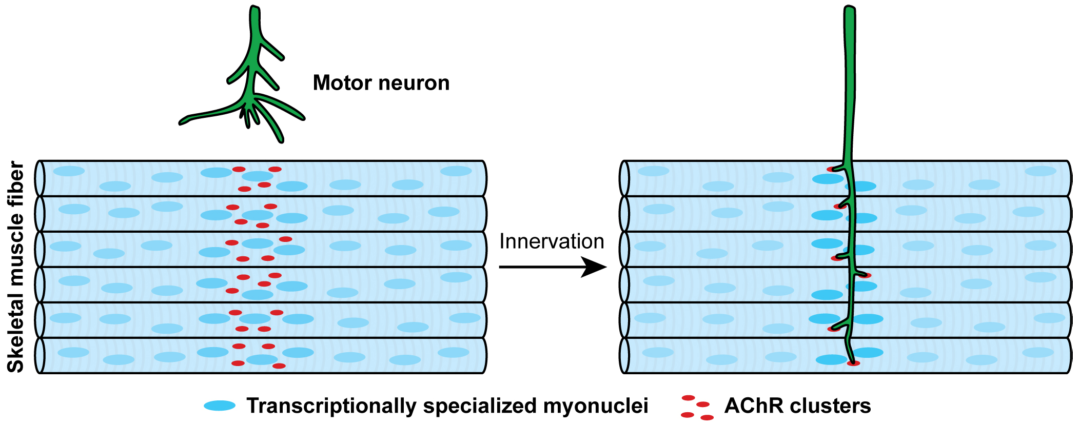
\includegraphics[width=\textwidth]{./Images/formation_jnm.png}
	\caption{Formation de la \gls{jnm}.} 
	\descfig{Figure issue de Burden \emph{et al.} 2018 \cite{Burden2018}.}
	\label{fig:FormaJNM}
\end{figure}

\todo{mettre avec section musk ?}
Cette accumulation de \glspl{achr}, comme d'un certain nombre de protéines synaptiques, est due à un récepteur particulier : \gls{musk}. Ce dernier joue un rôle clef dans la formation de la synapse, sa position déterminant la position de cette dernière \cite{DeChiara1996, Glass1996}. Le ligand activateur de \gls{musk} est historiquement l'Agrine \cite{Glass1996}, qui est sécrété par l'axone au contact de la cellule musculaire. Plus récemment, des travaux ont montré que l'Agrine se fixait sur le co-récepteur de \gls{musk} : le récepteur \gls{lrp}4 \cite{Zhang2008, Kim2008}. Suite à l'activation par l'Agrine de \acrshort{lrp}4, deux complexes \gls{musk}/\gls{lrp}4 vont s'assembler, et cet assemblage tétramérique permettrait une phosphorylation optimale de \gls{musk}, et donc une différenciation complète de la synapse et de l'agrégation des \gls{achr} \cite{Zong2012}.

\section{Le récépteur \acrshort{musk}, une molécule clef de la synaptogénèse}
\label{sec:IntroMuSK}

\begin{wrapfigure}{l}{0.25\textwidth}
	\centering{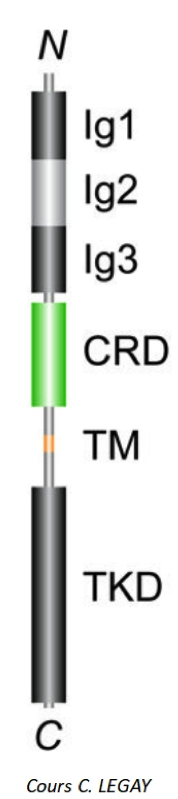
\includegraphics[width=0.1\textwidth]{./Images/MuSKReceptor.png}}
	\caption{Récepteur \gls{musk}}
	\descfig{Ig : Domaine immunoglobuline, CRD : \emph{Cysteine Rich Domain}, TM : Domaine transmembranaire,TKD : Domaine tyrosine kinase.}
	\label{fig:RMuSK}
\end{wrapfigure}

\acrfull{musk} est un récepteur découvert dans l'organe électrique de la raie \emph{Torpedo california} \cite{Jennings1993}. L'expression de ce récepteur à d'abord été mesurée dans les cellules musculaires et localisée au niveau de la \gls{jnm}. \gls{musk} est une récepteur tyrosine-kinase de 98kDa, dans lequel on distingue trois parties : un ectodomaine (partie N-terminale), un domaine transmembranaire, et un domaine cytoplasmique qui porte l'activité kinasique (voir \cref{fig:RMuSK}). 

La partie extracellulaire comporte généralement trois domaines \gls{ig}, dont le domaine \gls{ig}1 a récemment été impliqué dans la liaison avec \gls{lrp}4 \cite{Zhang2011}, ainsi qu'un domaine Frizzled-like, riche en cystéines (\gls{crd}) \cite{Jing2009}.

\gls{musk} possède trois ligands connus : l'Agrine (via \acrshort{lrp}4), un collagène spécifique associé à l'\Gls{ache} appelé \acrshort{colq}, et les \Glspl{wnt}, tous nécessaire au développement complet de la synapse. Un défaut de signalisation de l'un d'entre eux entraîne ainsi des défauts structuraux et/ou fonctionnels de la synapse.

La présence de \gls{musk} dans le cerveau a longtemps été ignorée, du fait de sa faible expression dans cette organe, quantifiée dans le passé par Northern Blot, une méthode de détection des \acrshort{arnm} peu sensible. Cependant, de nouvelles techniques, telle que l'\gls{his} ou bien la \gls{qpcr}, ont permis de montrer que le récepteur était bien présent dans le tissu cérébral, principalement au niveau des neurones du cortex, du cervelet, et de l'hippocampe \cite{Garcia-Osta2006, Ksiazek2007}. Le récepteur \gls{musk} est exprimé aussi dans les astrocytes \cite{Sun2016}, à des taux jusqu'à 5 fois supérieur à son expression dans les muscles squelettiques, où avec son co-récepteur \gls{lrp}4 il régulerait la transmission glutamatergiques au travers du relargage d'ATP et une signalisation liée à l'agrine.

Au niveau du \gls{snc}, deux isoformes de \gls{musk} semblent être exprimées \cite{Garcia-Osta2006}. La première isoforme, de 2644pbs, est identique à une isoforme générée par épissage alternatif dans le muscle \cite{Valenzuela1995}, sans qu'aucun rôle ne lui soit connu pour l'instant. La seconde isoforme est plus courte : 2359pbs, et présente une délétion du troisième domaine \gls{ig}. Les deux isoformes présentent une alanine à la position 454 qui remplace une délétion de 8a.a de l'éctodomaine. Une autre isoforme ayant le domaine \gls{ig}3 supprimé serait impliquée dans l'agrégation des \gls{achr} \cite{Hesser1999}.

Grâce à des techniques de knockdown du gène par séquence antisens au niveau de l'hippocampe, il apparaîtrait que la présence de \gls{musk} dans le cerveau serait nécessaire mais non indispensable à la formation de la mémoire à moyen et long-terme \cite{Garcia-Osta2006}. La voie \gls{creb} est une voie impliquée dans la formation de la mémoire au niveau de l'hippocampe \cite{Silva1998, Kandel2012,Kida2014,Ortega-Martinez2015}, qui passerait par la phosphorylation de \gls{creb} suite au relargage de \acrshort{camp}, augmentant son activité transcriptionnelle. Un modèle propose \cite{Garcia-Osta2006} que l'activation de \gls{musk} activerait la cascade de signalisation de \gls{creb}, permettant la consolidation de la mémoire. Ce modèle expliquerait également l'auto-régulation de \gls{musk} \cite{Moore2001}, dont le gène possède dans sa séquence promotrice un élément CRE-like liant \gls{creb} \cite{Kim2005}. De plus, \gls{musk} est nécessaire à la formation de la \gls{ltp} de l'hippocampe \cite{Garcia-Osta2006}.

\todo{faire transition musk wnt}

\section{Les protéines \Acrshortpl{wnt}, ligands de \acrshort{musk}}
\label{sec:IntroWnt}

\begin{wrapfigure}{l}{0.4\textwidth}
	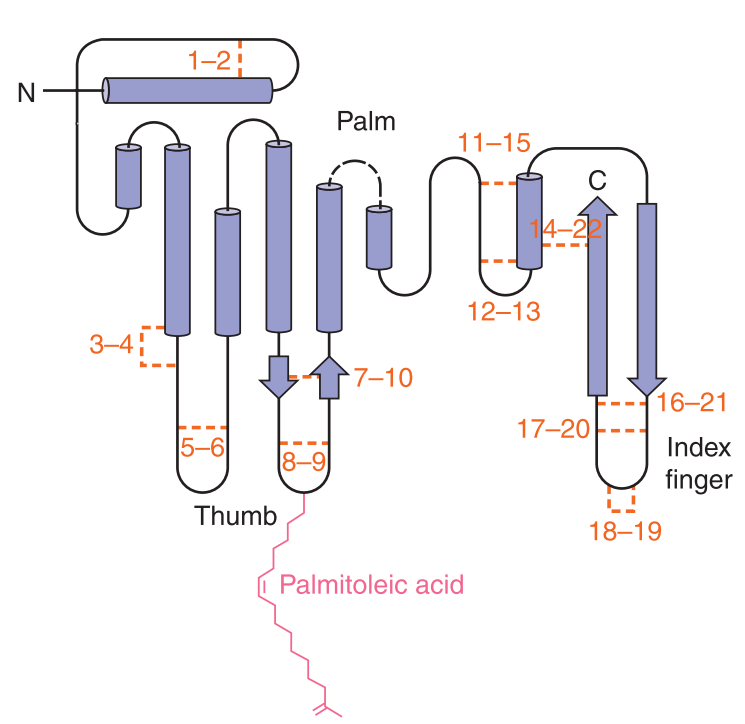
\includegraphics[width=0.4\textwidth]{./Images/WntProtein.png}	
	\caption{Structure d'une protéine \Gls{wnt} classique.}
	\descfig{Figure issue de Willert \& Nusse 2012 \cite{Willert2012}. En orange sont représentés les 22 résidus cystéines.}
	\label{fig:WntProt}
\end{wrapfigure}

Les protéines \gls{wnt} sont des glycoprotéines sécrétées, de 40kDa pour 350 acides aminés, impliquées dans de nombreux processus développementaux tel que l'embryogenèse, la prolifération, la différenciation, la migration cellulaire, ou encore l'apoptose \cite{Miller2002, Willert2012}. La structure des \Glspl{wnt} est complexe, avec  de nombreux ponts disulfures caractéristiques de cette famille de protéines, d'hélices \textalpha{}, ainsi que la présence d'un acide palmitoléïque participant à la liaison avec le récepteur (voir \cref{fig:WntProt}). On peut également souvent observé la présence d'un acide palmitique conservé au cours de l'évolution. La présence de ces acides gras rendent les protéines \Gls{wnt} très hydrophobes, ce qui a retardé leurs caractérisations.

En plus de leurs rôles durant le développement, les \Glspl{wnt} jouent également un rôle à l'age adulte dans la maintenance des tissus adultes. Des travaux ont pu montré que les \Glspl{wnt} étaient également impliquées dans des étapes précoces de la formation de la \gls{jnm} \cite{Hall2000}. On connaît actuellement 19 membres de cette famille de protéine chez la souris et chez l'humain. Classiquement, les \Glspl{wnt} se lient sur le domaine \gls{crd} de leur récepteur \gls{fz}, associé aux co-récepteurs \gls{lrp}5 ou 6, mais il existe d'autres récepteurs non canoniques tels que : \gls{ror} \cite{Cadigan2006, Gordon2006, Green2008}, \gls{ryk} \cite{Bovolenta2006, Fradkin2010}, ou bien encore \gls{musk} \cite{Jing2009}, qui possèdent également un \gls{crd}.

Il a été montré \emph{in vitro} que plusieurs \Glspl{wnt} interagissaient avec \gls{musk} : \Gls{wnt}2, 3a, 4, 6, 7b, 9a, et 11 \cite{Strochlic2012, Zhang2012, Barik2014}, avec différents effets. Seules \gls{wnt}4, 9a et 11 vont conduire à une dimérisation de \gls{musk} et a son activation (\emph{in vitro}). Ceci est cohérent avec le fait que chez le Poisson-zèbre, l'orthologue de \gls{musk}, \emph{unplugged}, possède un \gls{crd} qui interagit avec des protéines \Glspl{wnt} pour induire l'agrégation de \glspl{achr} \cite{Jing2009, Gordon2012}. \Gls{lrp}4 semble être également nécessaire à l'agrégation des \gls{achr} médié par les \gls{wnt}s \cite{Zhang2012}.

Les protéines \gls{wnt} peuvent activer plusieurs voies de signalisation différentes dans la cellule :  la voie canonique/\textbeta{}-catenin, la voie \gls{pcp}, et d'autres voies indépendante de la \textbeta{}-catenin. Pour la voie canonique, en l'absence de \Glspl{wnt} sur le récepteur \gls{fz}, la \textbeta{}-catenin est continuellement reconnue par le complexe \acrshort{gsk3}-\acrshort{apc}-\acrshort{ck1}. Ce complexe va phosphorylé la \textbeta{}-catenin, permettant sa reconnaissance par la \gls{btrcp}, une E3 ubiquitine-ligase et son marquage pour destruction par le protéasome. Quand les \Glspl{wnt} se lient à \emph{\gls{fz}}, \emph{Dishevelled} (une protéine centrale dans les différentes voie \gls{wnt} \cite{Gao2010}) est recrutée à la membrane, permettant l'interaction de \gls{lrp}5/6 avec la \gls{gsk3}. Cette interaction va libéré la \textbeta{}-catenin qui s'accumule dans le cytoplasme, puis se translocalise dans le noyau, d'où elle va avoir un effet sur la transcription des gènes. 

La voie \gls{pcp} est impliquée principalement dans la migration, la polarisation et le destin cellulaire. Cette voie dans le \gls{snc} est essentielle pour la gastrulation et la formation du tube neural durant l'embryogenèse \cite{Adler2002, Nejsum2009}. La voie \gls{pcp} est très complexe, de nombreux acteurs de cette voie sont également impliqués dans d'autres voies de signalisations importantes. Les \Glspl{wnt} en se liant à \gls{fz} vont recrutés \emph{Dishevelled} à la membrane, conduisant à l'activation de \acrshort{rhoa} et \gls{rock}. L'activation de ces protéines va entrainé le remodelage du cytosquelette d'actine et du réseau microtubulaire, nécessaire à la morphogénèse cellulaire. La voie \gls{pcp} active également \acrshort{jnk} et c-JUN activant la transcription de gènes cibles \cite{Niehrs2012}.

Enfin, parmi les voies \glspl{wnt} non canonique, la plus connue est la voie \Gls{wnt}/Calcium, ou \emph{Dishevelled} va activer la \acrshort{plc}, résultant en une augmentation de la concentration intracellulaire d'\acrshort{ip3} et de \acrshort{dag}. L'\acrshort{ip3} provoque l'ouverture des canaux calciques du \gls{re}. Cette augmentation de calcium active la \acrshort{pkc} et la \acrshort{campk2}, qui vont agirent sur la transcription nucléaires au travers de différents facteurs tels que \acrshort{creb} \cite{Koles2012}. De plus, il a été montré que dans certains cas en réponse à une stimulation par \Gls{wnt}3, le récepteur \gls{ryk} était clivé par la \textgamma{}-sécrétase, induisant la translocation de la partie intracellulaire du récepteur dans le noyau \cite{Lyu2008}.

\section{\acrshort{musk} dans le cerveau}
\label{sec:MuSKCerveau}

Texte

\section{\acrshort{musk} et \Acrshortpl {wnt} : Contexte de l'étude et but du stage}
\label{sec:Contexte}

Dans le but d'étudier le rôle de l'interaction des protéines \Glspl{wnt} et du domaine \gls{crd} de \gls{musk}, l'équipe de C. LEGAY à crée une souris transgénique dont le \gls{crd} était supprimé (\mcrd) \cite{Messeant2015, Messeant2017}. Il a ainsi été montré que le \gls{crd} était nécessaire à la \gls{jnm} à la fois pour sa formation et pour son maintien à l'age adulte, et que \Gls{wnt}4 et 11 participaient activement à la formation de cette dernière. De plus, un traitement au \gls{licl} (inhibiteur de la \gls{gsk3}) permettait à la \gls{jnm} un retour vers un phénotype sauvage. 

En plus de leurs problèmes musculaires, les souris \mcrd exhibaient des défauts centraux : durant son stage, une étudiante, Bertille SOMON, a montré que les mutants mâles avaient des blessures importantes au niveau du dos, blessures qui n'étaient pas dues à des comportements d'agressivité entre souris. De plus, une analyse comportementale a été réalisée en collaboration avec le groupe du Dr LANFUMEY (Centre de Psychiatrie et Neurosciences, Paris), et le test \gls{nor} a révélé que les souris mutantes souffraient d'un déficit de la mémoire intermédiaire.

Comme \gls{musk} est exprimé dans le cerveau adulte, principalement au niveau de l'hippocampe \cite{Garcia-Osta2006}, et que ce lieu joue un rôle prépondérant dans la formation de la mémoire intermédiaire, l'objectif de mon stage va être d'explorer le rôle de l'interaction de \gls{musk} et des \Glspl{wnt} dans le cerveau, utilisant pour cela les souris \mcrd.

Cela se fera au travers de 5 axes : 
\begin{enumerate}
	\item \sout{Quelle est l'origine des blessures chez le mâle ?}
	\item La structure du cerveau est-elle affectée chez le mutant ?
	\item Quelles sont les cellules exprimant \gls{musk} ?
	\item Quel est le niveau d'expression de \gls{musk}/\mcrd dans le cerveau ?
	\item \sout{Un traitement au \gls{licl} peut-il permettre un retour du mutant à un phénotype sauvage au niveau du comportement ?}
\end{enumerate}